\documentclass[tikz, border=2pt]{standalone}
\usepackage{amsmath}

\begin{document}
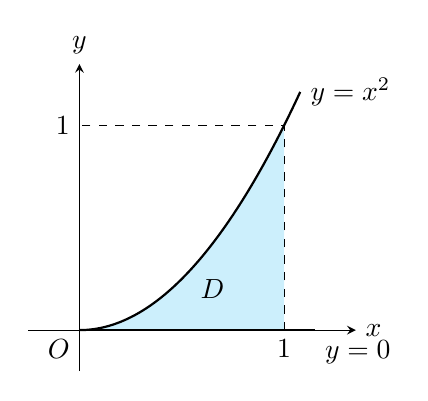
\begin{tikzpicture}[scale=2.6, >=stealth]
    % D bounded by y=0, y=x^2 and x=1
    \fill[cyan!20] (0,0) -- plot[domain=0:1, samples=80] (\x,{\x*\x}) -- (1,0) -- cycle;

    \draw[->] (-0.25,0) -- (1.35,0) node[right] {$x$};
    \draw[->] (0,-0.2) -- (0,1.3) node[above] {$y$};

    \draw[thick, domain=0:1.08, samples=100] plot (\x,{\x*\x}) node[right] {$y=x^2$};
    \draw[thick] (0,0) -- (1.15,0) node[below right] {$y=0$};
    \draw[dashed] (1,0) node[below] {$1$} -- (1,1) -- (0,1) node[left] {$1$};

    \node[below left] at (0,0) {$O$};
    \node at (0.65,0.2) {$D$};
\end{tikzpicture}
\end{document}
